%\VignetteIndexEntry{Using stm}
%\documentclass[nojss]{jss}
\documentclass[article,shortnames]{jss}

\author{\hspace{1.1in}Margaret E. Roberts\\\hspace{1.1in}UCSD \And
  \hspace{1.5in}Brandon M. Stewart\\\hspace{1.5in}Princeton \And
  \hspace{1.5in}Dustin Tingley\\\hspace{1.5in}Harvard \And
}
\title{\pkg{stm}: \proglang{R} Package for Structural Topic Models}

\Plainauthor{Margaret E. Roberts, Brandon M. Stewart, Dustin Tingley} %% comma-separated
\Plaintitle{stm: R Package for Structural Topic Models} %% without formatting
\Shorttitle{Structural Topic Models}  %% a short title (if necessary)

\Abstract{
This vignette demonstrates how to use the Structural Topic Model \pkg{stm} \texttt{R} package. The Structural Topic Model allows researchers to flexibly estimate a topic model that includes document-level meta-data. Estimation is accomplished through a fast variational approximation based approach. The \pkg{stm} package provides many useful features, including rich ways to explore topics, appropriate uncertainty estimation, and extensive plotting and visualization options.
}

\Keywords{structural topic model, text analysis, LDA, \pkg{stm}, \proglang{R}}
\Plainkeywords{structural topic model, text analysis, LDA, stm, R} %% without formatting

\Address{
  Margaret E. Roberts\\
  Department of Political Science\\
  University of California, San Diego\\
  Social Sciences Building 301\\
  9500 Gillman Drive, 0521, La Jolla, CA, 92093-0521 \\
  E-mail: \email{meroberts@ucsd.edu}\\
  URL: \url{http://www.margaretroberts.net}\\
  \\
  Brandon M. Stewart\\
  Department of Sociology\\
  Princeton University\\
  106 Wallace Hall, Princeton, NJ 08544 \\
  E-mail: \email{bms4@princeton.edu}\\
  URL: \url{brandonstewart.org}\\
\\
  Dustin Tingley\\
  Department of Government\\
  Harvard University\\
  1737 Cambridge St, Cambridge, MA, USA\\
  E-mail: \email{dtingley@gov.harvard.edu}\\
  URL: \url{http://scholar.harvard.edu/dtingley}\\

}


% == BibTeX packages
\usepackage{natbib}

% == Other Packages
\usepackage{amsmath, amsfonts, amssymb, url, bm}
\usepackage{rotating}
\usepackage{latexsym}
\usepackage{graphicx}
\usepackage{ulem}

\usepackage{placeins}

% == New Commands
% = For general typesetting
\newcommand\spacingset[1]{\renewcommand{\baselinestretch}{#1}\small\normalsize}

\setkeys{Gin}{width=0.5\textwidth}

\def\citepos#1{\citeauthor{#1}'s (\citeyear{#1})}
\newcommand\citea{\citeauthor}

\usepackage{Sweave}
\begin{document}
\Sconcordance{concordance:stmVignette.tex:stmVignette.Rnw:%
1 68 1 1 0 3 1 1 4 66 1 1 5 16 1 1 2 1 0 1 1 3 0 1 2 19 1 1 2 %
1 0 1 2 4 0 1 2 26 1 1 4 6 0 1 2 2 1 1 2 4 0 1 2 13 1 1 4 6 0 %
1 2 4 1 1 2 5 0 1 2 6 1 1 2 4 0 1 2 7 1 1 3 5 0 1 2 20 1 1 2 %
21 0 1 2 6 1 1 3 2 0 1 2 4 0 1 2 1 1 1 9 3 1 1 2 1 0 2 1 4 0 1 %
2 15 1 1 2 1 0 1 2 4 0 1 2 11 1 1 2 5 0 1 2 19 1 1 8 11 0 1 2 %
12 1 1 3 2 0 1 2 1 0 1 1 1 2 5 0 1 2 9 1 1 4 6 0 1 2 5 1 1 2 5 %
0 1 2 8 1 1 2 5 0 1 2 10 1 1 4 6 0 1 2 2 1 1 3 2 0 1 5 3 0 1 5 %
3 0 1 2 5 0 1 2 14 1 1 2 5 0 1 2 8 1 1 2 4 0 1 2 3 1 1 2 5 0 1 %
2 38 1 1 4 7 0 1 2 49 1 1 2 1 0 1 1 3 0 1 2 2 1 1 2 4 0 1 2 1 %
1 1 2 1 0 1 6 5 0 1 1 3 0 1 2 1 1 1 3 2 0 1 2 4 0 1 2 88 1}

\spacingset{1}

%%%%%%%%%%%%%%%%%%%%%%%%%%%%%%%%%%%%%%%%%%%%%%%%%%%%%%%%%%%%%%%%%%%%%%%%%%%%%%%%
\section{Introduction}

Text data is ubiquitious in social science research: traditional media, social media, survey data, and numerous other sources contribute to the massive quantity of text in the modern information age. The mounting availability of and interest in text data has been the development of a variety of statistical approaches for analyzing this data. We focus on the Structural Topic Model (STM), and its implementation in the \pkg{stm} \texttt{R} package,  which provides users tools for machine-assisted reading of large text corpora.\footnote{We thank Antonio Coppola, Jetson Leder-Luis, Christopher Lucas, and Alex Storer for various assistance in the construction of this package.  We also thank the many package users who have written in with bug reports and feature requests. Additional details and development version at \url{structuraltopicmodel.com}}  Building off of the tradition of probabilistic topic models, such as the Latent Dirichlet Allocation (LDA) \citep{blei2003latent} and Correlated Topic Model (CTM) \citep{blei2007correlated}, the Structural Topic Model's key innovation is that it permits users to incorporate \emph{metadata}, defined as information about each document, into the topic model. With the STM, users can model anything from the framing of international newspapers \citep{stmjasa}, open ended survey responses in the American National Election Study results \citep{ajps}, to online class forums \citep{StudentText}, to Twitter feeds and religious statements \citep{TextComparative}, to lobbying reports \citep{sailing}.\footnote{A fast growing range of other papers also utilize the model in a variety of ways \citep{wang2015time,goodman2015creating,fearfriction,constituent,chuangcomputer,TvinnereimClimate}.}


The goal of the Structural Topic Model is to allow researchers to discover topics and estimate their relationship to document metadata. Outputs of the model can be used to conduct hypothesis testing about these relationships. This of course mirrors the type of analysis that social scientists perform with other types of data, where the goal is to discover relationships between variables and test hypotheses. Thus the methods implemented in this paper help to build a bridge between statistical techniques and research goals. However, the \pkg{stm} package also provides tools to assist with a wide range of the work flow associated with analyzing textual data. The design of the package is such that users have a broad array of options to process raw text data, explore and analyze the data and present findings using a variety of plotting tools.

The outline of this paper is as follows. In Section~\ref{sec:est} we introduce the technical aspects of the STM, including the data generating process and an overview of estimation.  In Section \ref{sec:use} we provide examples of how to use the model and the package \texttt{stm}, including implementing the model and plots to visualize model output. Sections~\ref{sec:defaults} and ~\ref{sec:priors} cover more advanced material on ways to modify aspects of estimation. Section~\ref{sec:performance} demonstrates the superior performance of our implementation over related alternatives.  Section~\ref{sec:conclusion} concludes and Appendix~\ref{sec:eval} discusses several more advanced features.

\section{The Structural Topic Model}
\label{sec:est}

We begin by providing a technical overview of the STM model. Later in the paper we discuss additional technical details. Like other topic models, the STM is a generative model. That means we define a data generating process for each document and then use the data to find the most likely values for the parameters within the model.  Figure~\ref{fig:stmoverview} provides a graphical representation of the model. The generative model begins at the top, with document ($D_1,D_2...)$, topic ($T_1,T_2...$), and topic/word ($w_1,w_2$...) distributions generating documents that have metadata associated with them ($X_d$, where $d$ indexes the documents). Within this framework (which is the same as other topic models like LDA), a topic is defined as a mixture over words where each word has a probability of belonging to a topic. And a document is a mixture over topics, meaning that a single document can be composed of multiple topics.\footnote{As such, the sum of the topic proportions across all topics for a document is one, and the sum of the topic probabilities for a word, across all topics, is one.}

Figure~\ref{fig:stmoverview} and the statement below of the document generative process highlight the case where topical prevalence and topical content can be a function of document metadata. Topical \emph{prevalence} refers to how much of a document is associated with a topic (described on the left hand side) and topical \emph{content} refers to the words used within a topic (described on the right hand side). Hence metadata that explain topical prevalence are referred to as topical prevalence covariates, and variables that explain topical content are referred to as topical content covariates. It is important to note, however, that the model allows using either topical prevalence covariates or a topical content covariate, or neither.\footnote{In the case of no covariates, the model reduces to a fast implementation of the Correlated Topic Model \citep{blei2007correlated}}

The generative process for each document (indexed by $d$) for a STM model with $k$ topics can be summarized as:

\begin{enumerate}
\item Draw the document-level attention to each topic from a logistic-normal generalized linear model based on document covariates $X_d$. \\
\begin{equation}\label{eqn:dgp1}
\vec{\theta}_d | X_d\gamma, \Sigma \sim \text{ LogisticNormal}(\mu = X_d\gamma, \Sigma)
\end{equation}
\item Form the document-specific distribution over words representing each topic ($k$) using the baseline word distribution ($m$), the topic specific deviation $\kappa_k$, the covariate group deviation $\kappa_g$ and the interaction between the two $\kappa_i$.\\
\begin{equation}\label{eqn:dgp2}
\beta_{d,k} \propto  \text{ exp}(m + \kappa_{k} + \kappa_{g_d} + \kappa_{i = (kg_d)})
\end{equation}
\item For each word in the document, ($n \in 1, \dots, N_d$):
\begin{itemize}
\item Draw word's topic assignment based on the document-specific distribution over topics.\\
\begin{equation}\label{eqn:dgp3}
z_{d, n} | \vec{\theta}_d \sim \text{ Multinomial}(\vec{\theta})
\end{equation}
\item Conditional on the topic chosen, draw an observed word from that topic.\\
\begin{equation}\label{eqn:dpg4}
 w_{d, n} | z_{d, n}, \beta_{d, k= z} \sim \text{ Multinomial}(\beta_{d, k = z})
\end{equation}
\end{itemize}
\end{enumerate}

To fit the model, we use a semi-collapsed variational Expectation-Maximization algorithm which upon convergence gives us estimates of the model parameters. Regularizing prior distributions are used for $\gamma, \kappa$, and (optionally) $\Sigma$, which help enhance interpretation and prevent overfitting. Further technical details are provided in additional manuscripts \citep{nips2013,stmjasa,ajps,TextComparative}.\footnote{Available \href{http://scholar.harvard.edu/files/bstewart/files/stmnips2013.pdf}{here}, \href{http://scholar.harvard.edu/files/dtingley/files/comparativepoliticstext.pdf}{here}, \href{http://scholar.harvard.edu/files/dtingley/files/topicmodelsopenendedexperiments.pdf}{here}, and \href{http://scholar.harvard.edu/files/dtingley/files/comparativepoliticstext.pdf}{here}.} In this paper, we provide brief interpretations of results, and we direct readers to the companion papers for complete applications.


\begin{figure}
  \centering
  \includegraphics[scale=.45]{STMdiagram.pdf}
  \caption{Heuristic description of generative process and estimation of the STM.}\label{fig:stmoverview}
\end{figure}

\FloatBarrier

\section{Using the Structural Topic Model}
\label{sec:use}

In this section we demonstrate the basics of using the package.\footnote{The \pkg{stm} package leverages functions from a variety of other packages, including \pkg{Rcpp} \citep{eddelbuettel2011rcpp}, \pkg{RcppArmadillo} \citep{RcppArmadillo}, \pkg{MatrixStats} \citep{MatrixStats}, \pkg{slam} \citep{slam}, \pkg{lda} \citep{lda}, \pkg{stringr} \citep{stringr}, \pkg{SnowballC} \citep{SnowballC}, \pkg{tm} \citep{meyer2008text}, \pkg{igraph} \citep{igraph}, \pkg{huge} \citep{huge}, \pkg{glmnet} \citep{friedman2010regularization}, \pkg{clue} \citep{hornik2005clue}, \pkg{wordcloud} \citep{wordcloud}, \pkg{KernSmooth} \citep{KernSmooth}, \pkg{geometry} \citep{geometry}, and \pkg{Rtsne} \citep{Rtsne}}. Figure~\ref{fig:stmreview} presents a heuristic overview of the package, which parallels a typical workflow. For each step we list different functions in the \pkg{stm} package that accomplish each task. First users ingest the data and prepare it for analysis. Next a structural topic model is estimated. As we discuss below, the ability to estimate the structural topic model quickly allows for the \emph{evaluation}, \emph{understanding}, and \emph{visualization} of results. For each of these steps we provide examples of some of the functions that are in the package and discussed in this paper. All of the functions come with help files, and examples, that can be accessed by typing ? and then the function's name.



\begin{figure}
  \centering
  \includegraphics[scale=.45]{Flowchart}
  \caption{Heuristic description of \pkg{stm} package features.}\label{fig:stmreview}
\end{figure}

\FloatBarrier



\subsection{Ingest: Reading and processing text data}


The first step is to load data into \texttt{R}. The \pkg{stm} package represents a text corpus in three parts: a \code{documents} list containing word indices and their associated counts,\footnote{A full description of the sparse list format can be found in the help file for \code{stm}.} a \code{vocab} character vector containing the words associated with the word indices, and a \code{metadata} matrix containing document covariates. In this section, we describe utility functions for reading text data into \texttt{R} or converting from a variety of common formats that text data may come in. Note that particular care must be taken to ensure that documents and their vocabularies are properly aligned with the metadata. Our functions automatically handle this process.




\subsubsection{Reading in data from a ``spreadsheet''}

A common way that researchers store text data alongside covariates related to the text is in a spreadsheet, with each row a separate observation and one column containing the text data. The recommended method for handling this data is through the \pkg{quanteda} package, which makes it easy to import text and associated meta-data, prepare the texts for processing, and convert the documents into a document-term matrix.\footnote{Previous versions of \pkg{stm} recommended the function \code{textProcessor}, but this is now deprecated.}  For example, users would first read in a .csv file that contains the textual data and associated metadata using native \proglang{R} functions, or load a pre-prepared dataframe as we do below.\footnote{Note that the model does not permit estimation when there are variables used in the model that have missing values. As such, it can be helpful to subset data to observations that do not have missing values for metadata that will be used in the STM model.}  In \pkg{quanteda}, these can be read using the \code{textfile} function and added to a corpus object using the \code{corpus} constructor function, which holds both the texts and the associated covariates in the form of document-level meta-data.

To illustrate how to use the \pkg{stm} package, we will use a collection of blogposts about American politics that were written in 2008, from the CMU 2008 Political Blog Corpus \citep{poliblog}.\footnote{The set of blogs is available at \url{http://sailing.cs.cmu.edu/socialmedia/blog2008.html} and documentation on the blogs is available at \url{http://www.sailing.cs.cmu.edu/socialmedia/blog2008.pdf}.  You can find the cleaned version of the data we used for this vignette here: \url{http://goo.gl/tsprNO}.} The blogposts were gathered from six different blogs: American Thinker, Digby, Hot Air, Michelle Malkin, Think Progress, and Talking Points Memo.  Each blog has its own particular political bent.  The day within 2008 when each blog was written was also recorded.  Thus for each blogpost, there is metadata on the day it was written and the political ideology of the blog for which it was written. In this case, each blog post is a row in a .csv file, with the text contained in a variable called ``documents''.


\begin{Schunk}
\begin{Sinput}
R> require(quanteda)
R> poliblogCorpus <- corpus(textfile("poliblogs2008.csv", textField = "documents"))
\end{Sinput}
\end{Schunk}


\subsubsection{Reading in data from other text processing programs}

Sometimes researchers will encounter data that is not in a spreadsheet format. The \pkg{quanteda} package contains very flexible tools for reading many formats of texts, such plain text, XML, and JSON formats and for easily creating a corpus from them.  We use the function \code{dfm} from the \pkg{quanteda} package to create the document term matrix that can be supplied directly to the \code{stmD} model fitting function.

An alternative program that is helpful for setting up and processing text data with document metadata, is \href{www.txtorg.org}{txtorg} \citep{TextComparative}. The \pkg{txtorg} program generates three separate files: a metadata file, a vocabulary file, and a file with the original documents. The default export format for \pkg{txtorg} is the \texttt{ldac} sparse matrix format popularized by David Blei's implementation of LDA.  The \code{readCorpus()} function can read in data of this type using the ``ldac'' option.

\subsubsection{Pre-processing text content}

It is often useful to engage in some processing of the text data before modelling it. The most common processing steps are stemming (reducing words to their root form) and stop word removal (e.g., ``the'', ``is'', ``at'').  The \pkg{quanteda} package can be used to implement stemming and stop word removal, and to reduce the size of the document-term matrix in a variety of flexible ways. 


\subsection{Prepare: Associating text with metadata}


After reading in the data, we suggest using the utility function \code{prepDocuments} to process the loaded data to make sure it is in the right format. In particular, the \code{prepDocuments} function properly associates metadata with text data and re-indexes this relationship when text data fields are blank or become blank following pre-processing (such as with stop word removal). Please see the help file for this function for more details.

\code{prepDocuments} also removes infrequent terms depending on user-set parameter \code{lower.thresh}. The utility function \code{plotRemoved} will plot the number of words and documents removed for different thresholds. For example, the user can use:

\begin{Schunk}
\begin{Sinput}
R> plotRemoved(processed$documents, lower.thresh = seq(1, 200, by = 100))
R> out <- prepDocuments(processed$documents, processed$vocab,
+  processed$meta, lower.thresh = 15)
\end{Sinput}
\end{Schunk}

to evaluate how many words and documents would be removed from the dataset at each word threshold, which is the minimum number of documents a word needs to appear in in order for the word to be kept within the vocabulary.  Then the user can select their preferred threshold within \code{prepDocuments}.
 

 


Importantly, \code{prepDocuments} also will re-index all metadata/document relationships if any changes occur due to processing. For example, if a document is completely removed due to pre-processing, then \code{prepDocuments} will make sure the correct metadata/document relationships hold. After reading in and processing the text data, it is important to inspect features of the documents and the associated vocabulary list to make sure they have been correctly preprocessed.

From here, researchers are ready to estimate a structural topic model.

\subsection{Estimate: Estimating the structural topic model}

The data import process will output documents, vocabulary and metadata that can be used for an analysis. In this section we illustrate how to estimate the STM. Next we move to a range of functions to evaluate, understand, and visualize the model.

%\subsubsection{Ways to use metadata}

The key innovation of the STM is that it incorporates metadata into the topic modeling framework.  In STM, metadata can be entered in the topic model in two ways: topical prevalence and topical content.  Metadata covariates for \emph{topical prevalence} allow the observed metadata to affect the frequency with which a topic is discussed.  Covariates in \emph{topical content} allow the observed metadata to affect the word rate use within a given topic--that is, how a particular topic is discussed. Estimation for both topical prevalence and content proceeds via the workhorse \code{stm} function.

\subsubsection{Estimation with topical prevalence parameter}

In this example, we use the ratings variable (blog ideology) as a covariate in the topic \emph{prevalence} portion of the model with the CMU Poliblog data described above. Each document is modeled as a mixture of multiple topics. Topical prevalence captures how much each topic contributes to a document. Because different documents come from different sources, it is natural then to want to allow this prevalence to vary with metadata that we have about document sources.

In this example we simply let prevalence be a function of the ``ratings'' variable, which is coded as either ``Liberal'' or ``Conservative,'' and the variable ``day.'' which is an integer measure of days running from the first to the last day of 2008. To illustrate, we now estimate a 20 topic STM model. The user can then pass the output from the model, \code{poliblogPrevFit}, through the various functions we discuss below (e.g., \code{plot.STM}) to inspect the results.

If a user wishes to specify additional prevalence covariates, she would do so using the standard formula notation in \proglang{R} which we discuss at greater length below. A feature of the \code{stm} function is that ``prevalence'' can be expressed as a formula that can include multiple covariates and factorial or continuous covariates.  For example, by using the formula setup we can enter other covariates additively. Additionally users can include more flexible functional forms of continuous covariates, including standard transforms like \code{log()}, as well as \code{ns()} or \code{bs()} from the \pkg{splines} package. The \pkg{stm} package also includes a convenience function \code{s()}, which selects a fairly flexible b-spline basis. In the current example we allow for the variable ``date'' to be estimated with a spline. As we show later in the paper, interactions between covariates can also be added using the standard notation for \texttt{R} formulas. In summary, in the example below, we enter in the variables additively, but allowing for the day variable, an integer variable measuring which day the blog was posted, to have a non-linear relationship in the topic estimation stage.

\begin{Schunk}
\begin{Sinput}
R> poliblogPrevFit <- stm(out$documents, out$vocab, K = 20,
+  prevalence =~ rating + s(day), max.em.its = 75,
+  data = out$meta, init.type = "Spectral")
\end{Sinput}
\end{Schunk}

The model is set to run for a maximum of 75 EM iterations (controlled by \code{max.em.its}) using a seed we selected (\code{seed}).  Typically, convergence of the model will be monitored by the change in the approximate bound between EM iterations.  Once the bound has a small enough change between iterations, the model is considered converged. To reduce compiling time, in this paper we do not run the models and instead load a workspace with the models already estimated.

\begin{Schunk}
\begin{Sinput}
R> load(url("http://goo.gl/VPdxlS"))
\end{Sinput}
\end{Schunk}

\subsection{Evaluate: Model selection and search}

\subsubsection{Model initialization for a fixed number of number of topics}

As with all mixed-membership topic models, the posterior is intractable and non-convex, which creates a multimodal estimation problem that can be sensitive to initialization. Put differently, the answers the estimation procedure comes up with may depend on starting values of the parameters (e.g., the distribution over words for a particular topic). There are two approaches to dealing with this that the \pkg{STM} package facilitates. The first is to use a specific intitialization based on the method of moments, which is deterministic and globally consistent under reasonable conditions \citep{chaptermulti}. This is known as a spectral initialization.\footnote{It uses a spectral decomposition (non-negative matrix factorization) of the word co-occurrence matrix.} In practice we have found this intialization to be very helpful. This can be chosen by setting \code{init.type = "Spectral"} in the \code{stm} function. We use this option in the above example. This means that no matter the seed that is set, the same results will be generated. However, it currently does not scale to extremely large vocabularies (uncommon in most applications) in which case alternative initializations are available, as we discuss below.

The second approach is to initialize the model with a short run of a collapsed Gibbs sampler for LDA. For completeness researchers can also initialize the model randomly, but this is generally not recommended. The default is \code{init.type = "LDA"} but in practice researchers on personal computers with vocabularies less that 10,000 can utilize the spectral initialization successfully.\footnote{When the initialization type is set to \code{"Spectral"} the user can specify \code{K=0} to use the algorithm of \cite{lee2014low} to select the number of topics.  The core idea of the spectral initialization is to approximately find the vertices of the convex hull of the word co-occurences.  The algorihm of \cite{lee2014low} projects the matrix into a low dimensional space using $t$-distributed stochastic neighbor embedding \citep{van2014accelerating} and then exactly solves for the convex hull.  This has the advantage of automatically selecting the number of topics.  The added randomness from the projection means that the algorithm is not deterministic as with the standard \code{"Spectral"} initialization type. Running it with a different seed can result in not only different results but a different number of topics.  We emphasize that this procedure has no particular statistical guarantees and should not be seen as estimating the ``true'' number of topics.  However it can be useful place to start.}


\subsubsection{Model selection for a fixed number of number of topics}

When the user cannot use the spectral initialization, she should estimate many models, each from randomly generated starting values, and then evaluate each \emph{model} according to some separate standard (we provide several below). The function \code{selectModel} automates this process to facilitate finding a model with desirable properties. Users specify the number of ``runs,'' which in the example below is set to 20. \code{selectModel} first casts a net where ``run'' (below 10) models are run for two EM steps, and then models with low likelihoods are discarded. Next, the default returns the 20\% of models with the highest likelihoods, which are then run until convergence or the EM iteration maximum is reached. Notice that options for the \code{stm} function can be passed to \code{selectModels}, such as \code{max.em.its}. If users would like to select a larger number of models to be run completely, this can also be set with an option specified in the help file for this function.

\begin{Schunk}
\begin{Sinput}
R> poliblogSelect <- selectModel(out$documents, out$vocab, K = 20,
+  prevalence =~ rating + s(day), max.em.its = 75,
+  data = out$meta, runs = 20, seed = 8458159)
\end{Sinput}
\end{Schunk}
In order to select a model for further investigation, users must choose one of the candidate models' outputs from \code{selectModel}. To do this, \code{plotModel} can be used to plot the average \emph{semantic coherence} and \emph{exclusivity} scores for each model (represented by topic numbers) as well as the semantic coherence and exclusivity for each topic.\footnote{See \citet{stmjasa,ajps} for a discussion of these criteria.} Each of these criteria are calculated for each topic within a model run. The \code{plotModel} function calculates the average across all topics for each run of the model and plots these by labeling the model run with a numeral. Often times users will select a model with desirable properties in both dimensions (i.e., models with average scores towards the upper right side of the plot). As shown in Figure~\ref{fig:select}, the \code{plotModel} function also plots each topic's values, which helps give a sense of the variation in these parameters.\footnote{For a given model, the user can plot the semantic coherence and exclusivity scores with the \code{topicQuality} function.}


\begin{figure}
\begin{center}
\begin{Schunk}
\begin{Sinput}
R> plotModels(poliblogSelect)
\end{Sinput}
\end{Schunk}
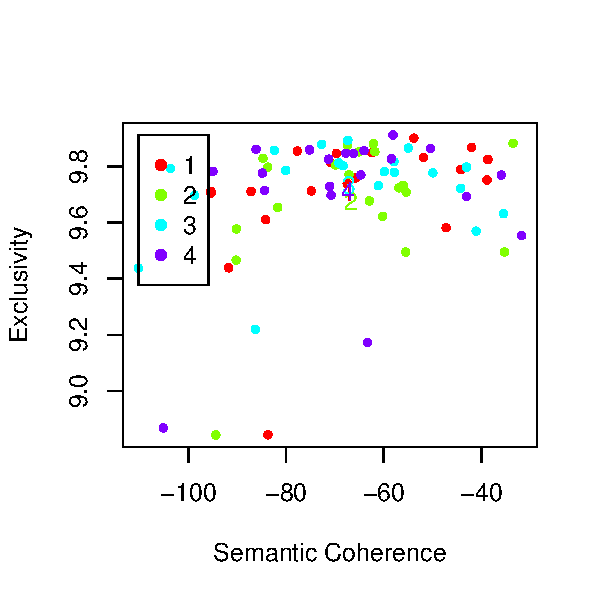
\includegraphics{stmVignette-008}
\caption{Plot of \code{selectModel} results. Numerals represent the average for each model, and dots represent topic specific scores.}
\label{fig:select}
\end{center}
\end{figure}

Next the user would want to select one of these models to work with. For example, the third model could be extracted from the object that is outputted by \code{selectModel}.

\begin{Schunk}
\begin{Sinput}
R> selectedmodel <- poliblogSelect$runout[[3]] 
\end{Sinput}
\end{Schunk}

Alternatively, as discussed in Section~\ref{sec:eval}, the user can evaluate the stability of particular \emph{topics} across models.  

\subsubsection{Model search across numbers of topics}

STM assumes a fixed user-specified number of topics. There is not a ``right'' answer to the number of topics that are appropriate for a given corpus, but the function \code{searchK} uses a data-driven approach to selecting the number of topics. The function will perform several automated tests to help choose the number of topics including calculating the held out likelihood \citep{wallach2009evaluation} and performing a residual analysis \citep{taddyestimation}. For example, one could estimate a STM model for 7 and 10 topics and compare the results along each of the criteria. The default initialization is the spectral initialization.  This function will also calculate a range of quantities of interest, including the average exclusivity and semantic coherence.\footnote{An alternative approach, useful when not using a spectral initialization, uses the \code{manyTopics} function which makes calls to the \code{stm} or the \code{selectModel} functions across multiple different numbers of topics. Note that in this case the process of extracting results differs from \code{selectModel} because results are stored in a list environment.}


\begin{Schunk}
\begin{Sinput}
R> storage <- searchK(out$documents, out$vocab, K = c(7, 10),
+  prevalence =~ rating + s(day), data = meta)
\end{Sinput}
\end{Schunk}


 
There are several other functions for evaluation shown in Figure~\ref{fig:stmreview}, and we discuss these in more detail in Appendix~\ref{sec:eval} so we can proceed with how to \emph{understand} and \emph{visualize} STM results.

\subsection{Understand: Interpreting the STM by plotting and inspecting results}

After choosing a model based on ex-ante criteria, the user must next interpret the model results. There are many ways to investigate the output, such inspecting the words associated with topics or the relationship between metadata and topics. To investigate the output of the model, the \pkg{stm} package provides a number of options.

\begin{enumerate}
\item Displaying words associated with topics (\code{labelTopics},\code{plot.STM(,type = "labels")}, \code{sageLabels},\code{plot.STM(,type = "perspectives")}) or documents highly associated with particular topics (\code{findThoughts},\code{plotQuote}).
\item Estimating relationships between metadata and topics/topical content (\code{estimateEffect}).
\item Calculating topic correlations (\code{topicCorr}).
\end{enumerate}

\subsubsection{Understanding topics through words and example documents}

We next describe two approaches for users to explore the topics that have been estimated. The first approach is to look at collections of words that are associated with topics. The second approach is to read actual documents that are estimated to be highly associated with each topic. Both of these approaches should be used. Below, we use the 20 topic model estimated with the spectral initialization.

To explore the words associated with each topic we can use the \code{labelTopics} function.  For models where a content covariate is included \code{sageLabels} can also be used. Both these functions will print to the monitor words associated with each topic. The function by default prints several different types of word profiles, including highest probability words and FREX words.\footnote{For more information on FREX and high probability rankings, see \citet{nips2013,stmjasa,ajps,TextComparative}. For more information on score, see the \pkg{lda} \proglang{R} package, \url{http://cran.r-project.org/web/packages/lda/lda.pdf}. For more information on lift, see \citet{taddy2012multinomial}.}  In order to translate these results to a format that can easily be used within a paper, the \code{plot.stm(,type = "labels")} function will print topic words to a graphic device. Notice that in this case, the labels option is specified as the \code{plot.STM} function has several functionalities that we describe below (the options for ``perspectives" and ``summary").

\begin{Schunk}
\begin{Sinput}
R> labelTopics(poliblogPrevFit, c(3, 7, 20))
\end{Sinput}
\begin{Soutput}
Topic 3 Top Words:
 	 Highest Prob: obama, barack, campaign, biden, polit, will, debat 
 	 FREX: ayer, barack, obama, wright, biden, jeremiah, joe 
 	 Lift: oct, goolsbe, ayerss, ayr, bernadin, ayer, annenberg 
 	 Score: oct, obama, barack, ayer, wright, campaign, biden 
Topic 7 Top Words:
 	 Highest Prob: palin, governor, sarah, state, alaska, polit, senat 
 	 FREX: blagojevich, palin, sarah, rezko, alaska, governor, gov 
 	 Lift: jindal, blagojevich, juneau, monegan, blago, burri, wasilla 
 	 Score: monegan, palin, blagojevich, sarah, alaska, rezko, governor 
Topic 20 Top Words:
 	 Highest Prob: bush, presid, administr, said, hous, white, report 
 	 FREX: cheney, tortur, cia, administr, interrog, bush, perino 
 	 Lift: addington, fratto, perino, mcclellan, feith, plame, cheney 
 	 Score: addington, bush, tortur, perino, cia, cheney, administr 
\end{Soutput}
\end{Schunk}

To read documents that are highly associated with topics the \code{findThoughts} function can be used. This function will print the documents highly associated with each topic.\footnote{The \code{theta} parameter in the \code{stm} object output has the posterior probability that this function uses.} Reading these documents is helpful for understanding the content of a topic and interpreting its meaning.

In our example, for expositional purposes, we restrict the length of the document to the first 200 characters.\footnote{This uses the object \code{shortdoc} contained in the workspace loaded above, which is the first 200 characters of original text.} We see that Topic 3 describes discussions of Obama during the 2008 presidential election. Topic 20 discusses the Bush administration.

To print example documents to a graphics device, \code{plotQuote} can be used. The results are displayed in Figure~\ref{fig:example}.

\begin{Schunk}
\begin{Sinput}
R> thoughts3 <- findThoughts(poliblogPrevFit, texts = shortdoc,
+  n = 2, topics = 3)$docs[[1]]
R> thoughts20 <- findThoughts(poliblogPrevFit, texts = shortdoc,
+  n = 2, topics = 20)$docs[[1]]
\end{Sinput}
\end{Schunk}

%manually correcting some unicode errors


\begin{figure}
\begin{center}
\begin{Schunk}
\begin{Sinput}
R> par(mfrow = c(1, 2),mar = c(.5, .5, 1, .5))
R> plotQuote(thoughts3, width = 30, main = "Topic 3")
R> plotQuote(thoughts20, width = 30, main = "Topic 20")
\end{Sinput}
\end{Schunk}
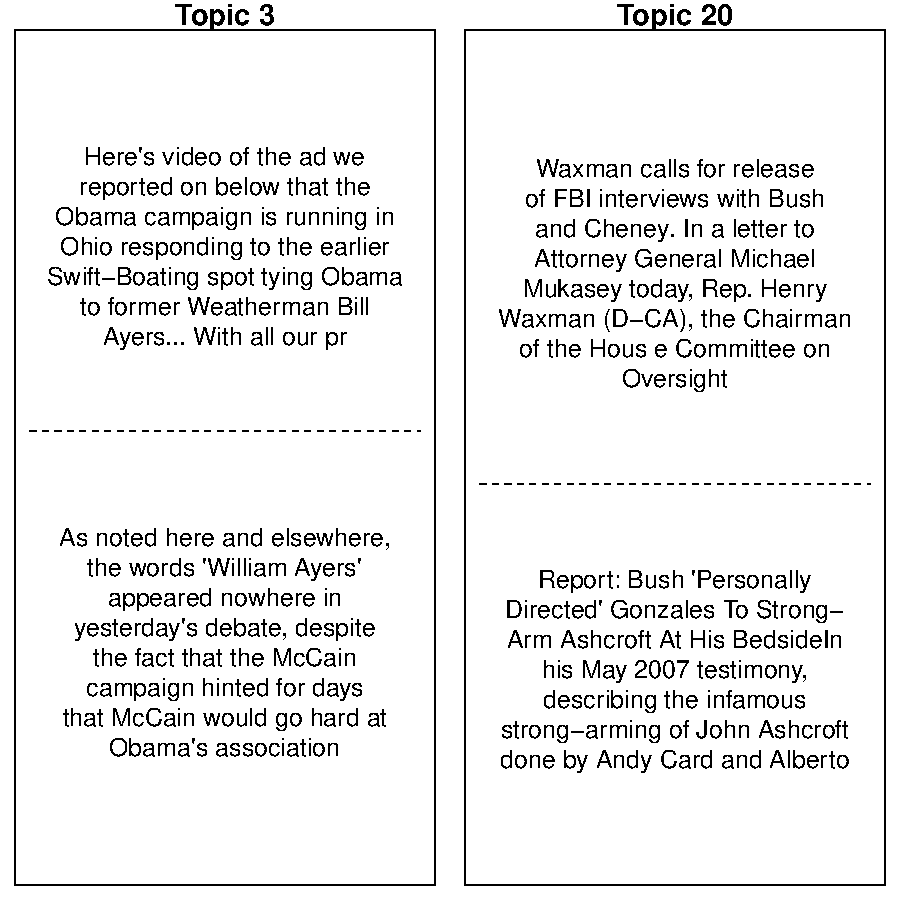
\includegraphics{stmVignette-014}
\caption{Example documents highly associated with topics 3 and 20.}
\label{fig:example}
\end{center}
\end{figure}



\subsubsection{Estimating metadata/topic relationships}

Estimating the relationship between metadata and topics is a core feature of the \pkg{STM} package. The workhorse function for estimating these relationships is \code{estimateEffect}. This function simulates a set of parameters which can then be plotted (which we discuss in great detail below). Typically, users will pass the same model of topical prevalence used in estimating the STM to the \code{estimateEffect} function. The syntax of the \code{estimateEffect} function is designed so users specify the set of topics they wish to use for estimation, and then a formula for metadata of interest. After the necessary method of composition simulations are done particular estimate strategies and standard plot design features can be used by calling the \code{plot.estimateEffect} function.


\code{estimateEffect} can calculate uncertainty in several ways. The default is ``global'', which will incorporate estimation uncertainty of the topic proportions into the uncertainty estimates using the method of composition. If users do not propagate the full amount of uncertainty, e.g., in order to speed up computational time, they can choose \code{uncertainty = "None"}, which will result in narrower confidence intervals because it will not include the additional estimation uncertainty.



\begin{Schunk}
\begin{Sinput}
R> out$meta$rating <- as.factor(out$meta$rating)
R> prep <- estimateEffect(1:20 ~ rating + s(day), poliblogPrevFit,
+  meta = out$meta, uncertainty = "Global")
\end{Sinput}
\end{Schunk}


\subsection{Visualize: Presenting STM results}

The functions we described previously to \emph{understand} STM results can be leveraged to \emph{visualize} results for formal presentation. In this section we focus on several of these visualization tools.

\subsubsection{Summary visualization}

Corpus level visualization can be done in several different ways. The first relates to the expected proportion of the corpus that belongs to each topic. This can be be plotted using \code{plot.stm(,type = "summary")}. An example from the political blogs data is given in Figure~\ref{fig:summary}. We see, for example, that the Sarah Palin/Vice President topic (7) is actually a relatively minor proportion of the discourse.  The most common topic, topic 3, is a general topic full of words that bloggers commonly use, and therefore is not very interpretable. The words listed in the figure are the top three words associated with the topic.

\begin{figure}
\begin{center}
\begin{Schunk}
\begin{Sinput}
R> plot.STM(poliblogPrevFit, type = "summary", xlim = c(0, .3))
\end{Sinput}
\end{Schunk}
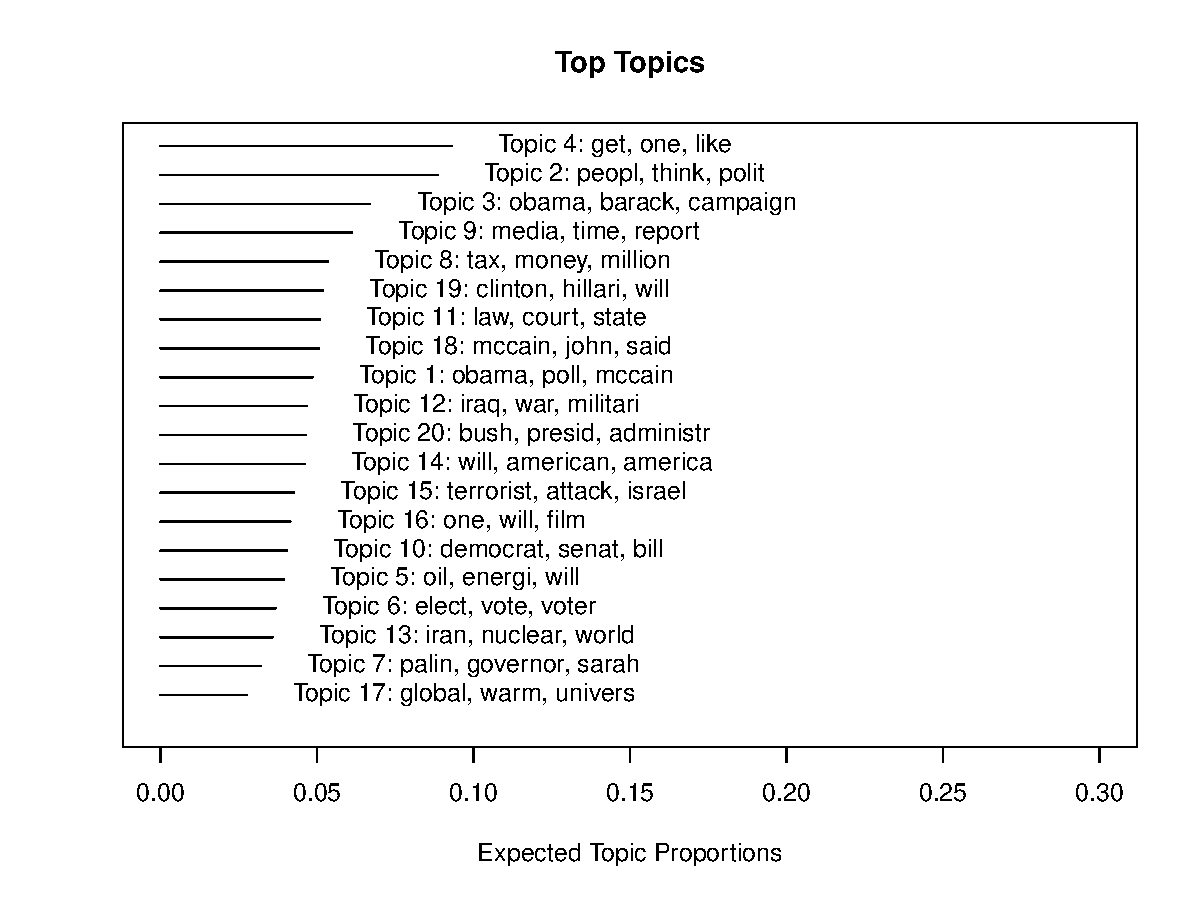
\includegraphics{stmVignette-016}
\caption{Graphical display of estimated topic proportions.}
\label{fig:summary}
\end{center}
\end{figure}


In order to plot features of topics in greater detail, there are a number of options in the \code{plot.STM} function, such as plotting larger sets of words highly associated with a topic or words that are exclusive to the topic. Furthermore, the \code{cloud} function will plot a standard word cloud of words in a topic and the \code{plotQuote} function provides an easy to use graphical wrapper such that complete examples of specific documents can easily be included in the presentation of results.

\subsubsection{Metadata/topic relationship visualization}

We now discuss plotting metadata/topic relationships in substantial detail, as the ability to estimate these relationships is a core advantage of the STM model. The core plotting function is \code{plot.estimateEffect}, which handles the output of \code{estimateEffect}.

First, users must specify the variable that they wish to use for calculating an effect. If there are multiple variables specified in \code{estimateEffect}, then all other variables are held at their sample median. These parameters include the expected proportion of a document that belongs to a topic as a function of a covariate, or a first difference type estimate, where topic prevalence for a particular topic is contrasted for two groups (e.g., liberal versus conservative).  \code{estimateEffect} should be run and the output saved before plotting when it is time intensive to calculate uncertainty estimates and/or because users might wish to plot different quantities of interest using the same simulated parameters from \code{estimateEffect}.\footnote{The help file for this function describes several different ways for uncertainty estimate calculation, some of which are much faster than others.} The output can then be plotted. %In this example we use a string variable and it is required that for this function that we first convert it into a factor variable.


When the covariate of interest is binary, or users are interested in a particular contrast, the method = "difference" option will plot the change in topic proportion shifting from one specific value to another. Figure~\ref{fig:difference} gives an example. For factor variables, users may wish to plot the marginal topic proportion for each of the levels (\code{"pointestimate"}).


\begin{figure}
\begin{center}
\begin{Schunk}
\begin{Sinput}
R> plot.estimateEffect(prep, covariate = "rating", topics = c(3, 7, 20),
+  model = poliblogPrevFit, method = "difference",
+  cov.value1 = "Liberal", cov.value2 = "Conservative",
+  xlab = "More Conservative ... More Liberal",
+  main = "Effect of Liberal vs. Conservative",
+  xlim = c(-.1, .1), labeltype = "custom",
+  custom.labels = c('Obama', 'Sarah Palin','Bush Presidency'))
\end{Sinput}
\end{Schunk}
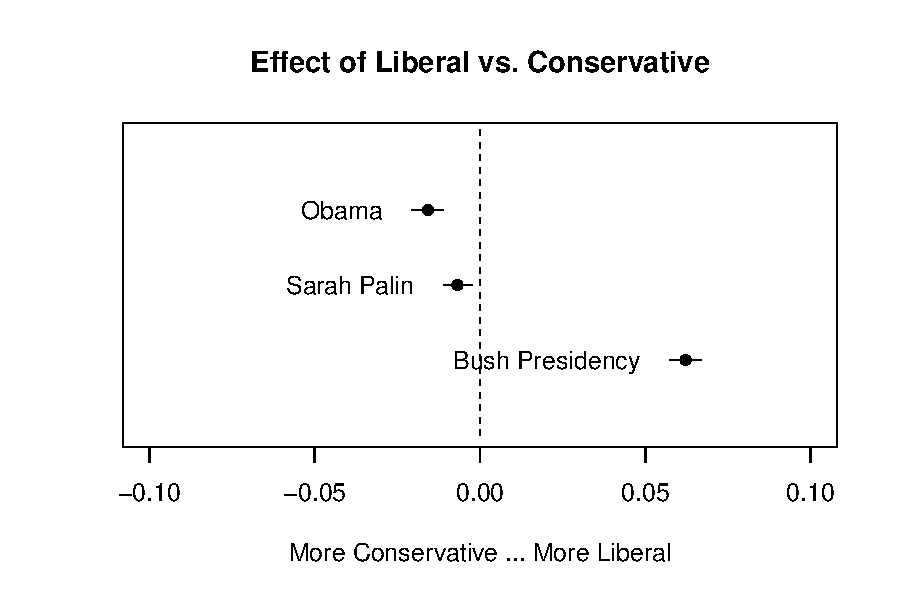
\includegraphics{stmVignette-017}
\caption{Graphical display of topical prevalence contrast.}
\label{fig:difference}
\end{center}
\end{figure}

We see Topic 1 is strongly used by conservatives compared to liberals, while Topic 7 is close to the middle but still conservative-leaning. Topic 10, the discussion of Bush, was largely associated with liberal writers, which is in line with the observed trend of conservatives distancing from Bush after his presidency.

Notice how the function makes use of standard labeling options available in the native plot() function. This allows the user to customize labels and other features of their plots. We note that in the package we leverage generics for the plot functions. As such, one can simply use \code{plot} instead of writing out the full extension (e.g., in Figure~\ref{fig:difference} one could use \code{plot} instead of \code{plot.estimateEffect}). For expositional purposes in this paper, we include the entire extension.

When users have variables that they want to treat continuously, users can choose between assuming a linear fit or using splines. In the previous example, we allowed for the day variable to have a non-linear relationship in the topic estimation stage. We can then plot its effect on topics. In Figure~\ref{fig:spline}, we plot the relationship between time and the vice presidential topic, topic 7.  The topic peaks when Sarah Palin became John McCain's running mate at the end of August in 2008.

\begin{figure}
\begin{center}
\begin{Schunk}
\begin{Sinput}
R> plot.estimateEffect(prep, "day", method = "continuous", topics = 7,
+  model = z, printlegend = FALSE, xaxt = "n", xlab = "Time (2008)")
R> monthseq <- seq(from = as.Date("2008-01-01"), 
+  to = as.Date("2008-12-01"), by = "month")
R> monthnames <- months(monthseq)
R> axis(1,at = as.numeric(monthseq) - min(as.numeric(monthseq)), 
+  labels = monthnames)
\end{Sinput}
\end{Schunk}
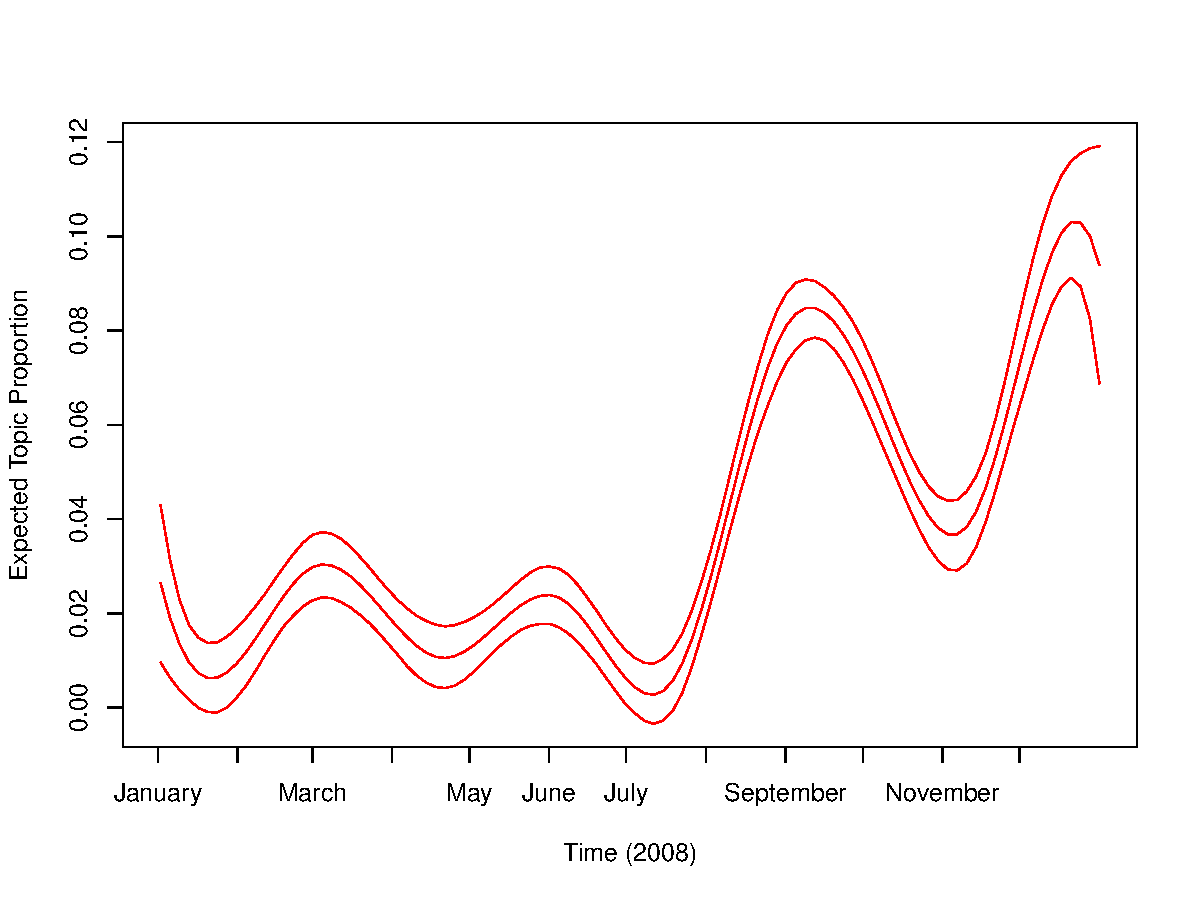
\includegraphics{stmVignette-018}
\caption{Graphical display of topic prevalence. Topic 7 prevalence is plotted as a smooth function of day, holding rating at sample median, with 95\% confidence intervals.}
\label{fig:spline}
\end{center}
\end{figure}


\subsubsection{Topical content}

We can also plot the influence of covariates included in as a topical content covariate. A topical content variable allows for the vocabulary used to talk about a particular topic to vary. First, the STM must be fit with a variable specified in the content option. In the below example, ratings serves this purpose. It is important to note that this is a completely new model, and so the actual topics may differ in both content and numbering compared to the previous example where no content covariate was used.

\begin{Schunk}
\begin{Sinput}
R> poliblogContent <- stm(out$documents, out$vocab, K = 20,
+  prevalence =~ rating + s(day), content =~ rating,
+  max.em.its = 75, data = out$meta, init.type = "Spectral")
\end{Sinput}
\end{Schunk}

Next, the results can be plotted using the \code{plot.STM(,type = "perspectives")} function.  This functions shows which words within a topic are more associated with one covariate value versus another. In Figure~\ref{fig:perp}, vocabulary differences by ratings is plotted for topic 11. Topic 11 is related to Guantanamo. Its top FREX words were ``tortur, detaine, court, justic, interrog, prosecut, legal''. However, Figure~\ref{fig:perp} lets us see how liberals and conservatives talk about this topic differently. In particular, liberals emphasized ``torture'' whereas conservatives emphasize typical court language such as ``illegal'' and ``law.'' \footnote{At this point you can only
 have a single variable as a content covariate, although that variable can have any number of groups. It cannot be continuous. Note that the computational cost of this type of model rises quickly with the number of groups and so it may be advisable to keep it small.}

\begin{figure}
\begin{center}
\begin{Schunk}
\begin{Sinput}
R> plot.STM(poliblogContent, type = "perspectives", topics = 11)
\end{Sinput}
\end{Schunk}
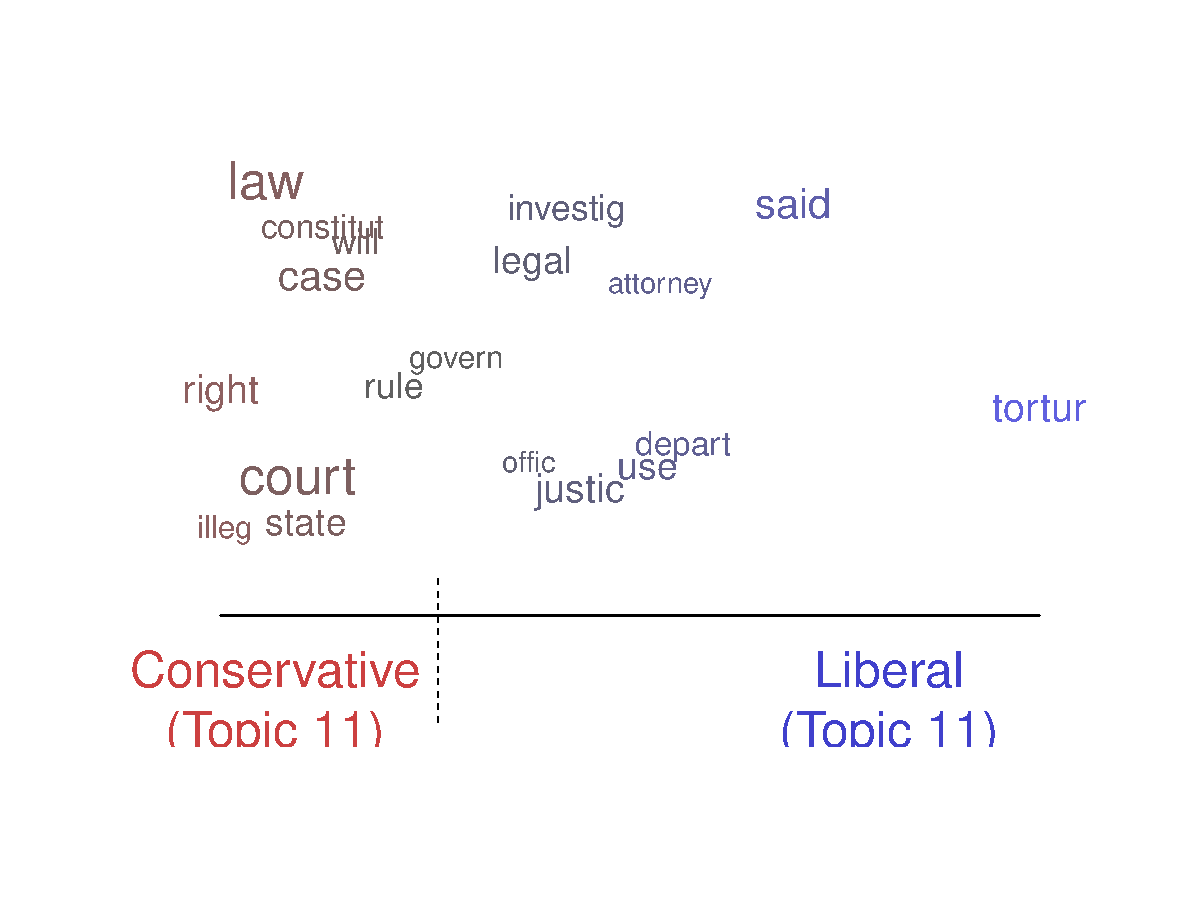
\includegraphics{stmVignette-020}
\caption{Graphical display of topical perspectives.}
\label{fig:perp}
\end{center}
\end{figure}

This function can also be used to plot the contrast in words across two topics.\footnote{This plot calculates the difference in probability of a word for the two topics, normalized by the maximum difference in probability of any word between the two topics.} To show this we go back to our original model that did not include a content covariate and we contrast topic 12 (Iraq war) and 20 (Bush presidency). We plot the results in Figure~\ref{fig:perp2}.

\begin{figure}
\begin{center}
\begin{Schunk}
\begin{Sinput}
R> plot.STM(poliblogPrevFit, type = "perspectives", topics = c(12, 20))
\end{Sinput}
\end{Schunk}
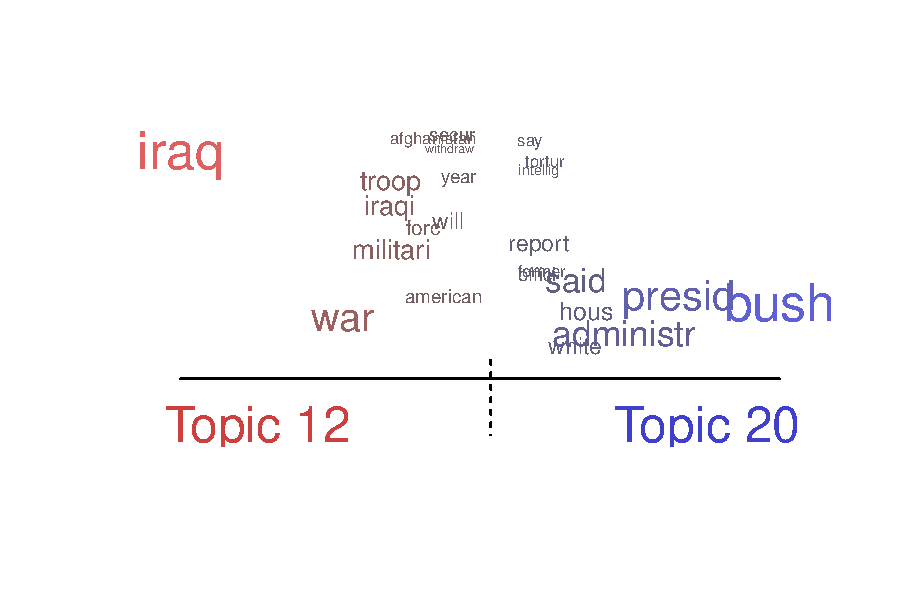
\includegraphics{stmVignette-021}
\caption{Graphical display of topical contrast between topics 12 and 20.}
\label{fig:perp2}
\end{center}
\end{figure}

\FloatBarrier

\subsubsection{Plotting covariate interactions}

Another modification that is possible in this framework is to allow for interactions between covariates such that one variable may ``moderate'' the effect of another variable. In this example, we re-estimated the STM to allow for an interaction between day (entered linearly) and ratings. Then in \code{estimateEffect()} we include the same interaction. This allows us in \code{plot.estimateEffect} to have this interaction plotted. We display the results in Figure~\ref{fig:spline2} for topic 20 (Bush administration). We observe that conservatives never wrote much about this topic, whereas liberals discussed this topic a great deal, but over time the topic diminished in salience.\footnote{Note that the ability to plot interactions only supports interactions with a binary effect modification covariate and does not support interactions with a spline.}

\begin{Schunk}
\begin{Sinput}
R> poliblogInteraction <- stm(out$documents, out$vocab, K = 20,
+  prevalence =~ rating * day, max.em.its = 75,
+  data = out$meta, init.type = "Spectral")
\end{Sinput}
\end{Schunk}

\begin{figure}
\begin{center}
\begin{Schunk}
\begin{Sinput}
R> prep <- estimateEffect(c(20) ~ rating * day, poliblogInteraction,
+  metadata = out$meta, uncertainty = "None")
R> plot.estimateEffect(prep, covariate = "day", model = poliblogInteraction,
+  method = "continuous", xlab = "Days", moderator = "rating",
+  moderator.value = "Liberal", linecol = "blue", ylim = c(0, .12),
+  printlegend = F)
R> plot.estimateEffect(prep, covariate = "day", model = poliblogInteraction,
+  method = "continuous", xlab = "Days", moderator = "rating",
+  moderator.value = "Conservative", linecol = "red", add = T,
+  printlegend = F)
R> legend(0, .08, c("Liberal", "Conservative"),
+  lwd = 2, col = c("blue", "red"))
\end{Sinput}
\end{Schunk}
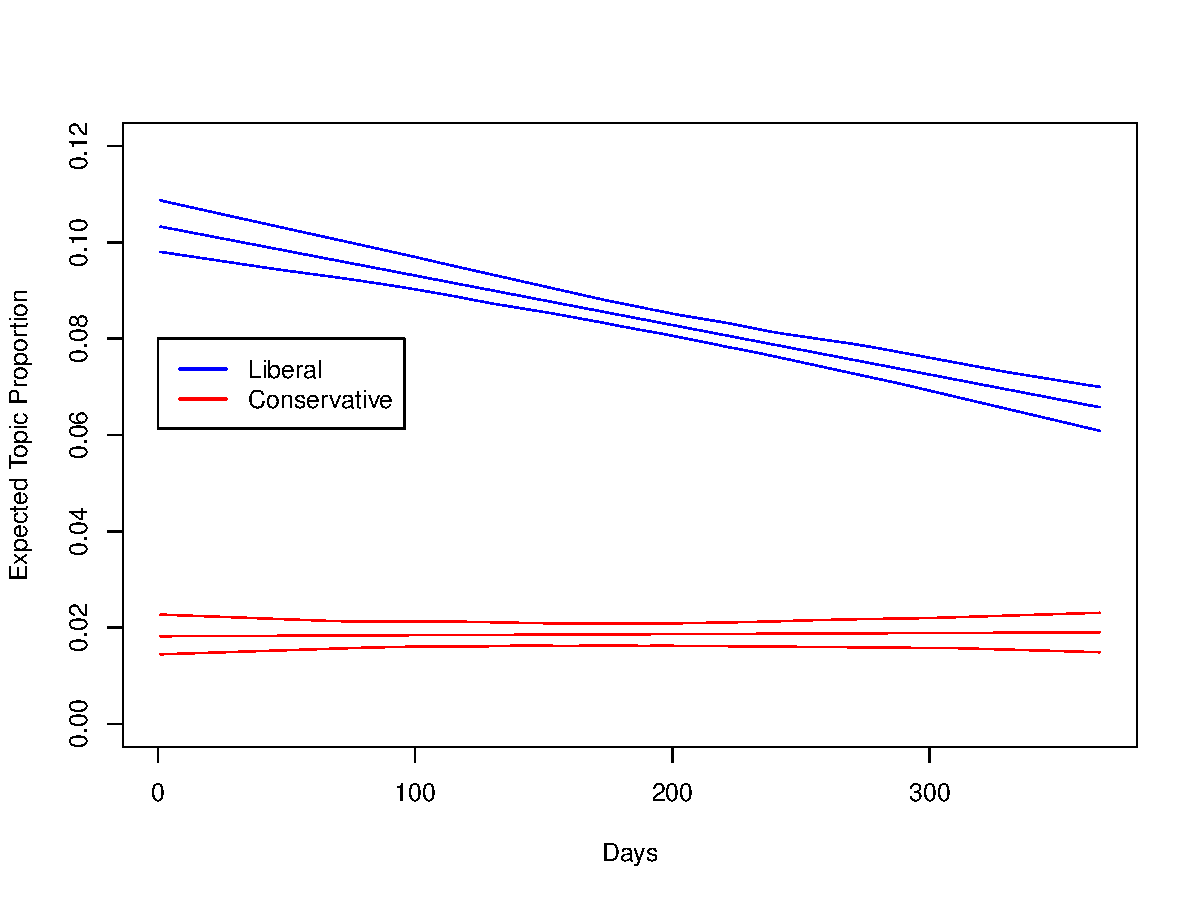
\includegraphics{stmVignette-023}
\caption{Graphical display of topical content. This plots the interaction between time (day of blog post) and rating (liberal versus conservative). Topic 20 prevalence is plotted as linear function of time, holding the rating at either 0 (Liberal) or 1 (Conservative). Were other variables included in the model, they would be held at their sample medians.}
\label{fig:spline2}
\end{center}
\end{figure}


More details are available in the help file for this function.\footnote{An additional option is the use of local local regression (loess). In this case, because multiple covariates are not possible a separate function is required, \code{plotTopicLoess}, which contains a help file for interested users.}.
\FloatBarrier
\subsection{Extend: Additional tools for interpretation and visualization}

There are multiple other ways to visualize results from an STM model. Topics themselves may be nicely presented as a word cloud. For example, Figure~\ref{fig:cloud} uses the \code{cloud} function to plot a word cloud of the words most likely to occur in blog posts related to the vice presidential candidates topic in the 2008 election.

\begin{figure}
\vspace{-20pt}
\begin{center}
\begin{Schunk}
\begin{Sinput}
R> cloud(poliblogPrevFit, topic = 7, scale = c(2,.25))
\end{Sinput}
\end{Schunk}
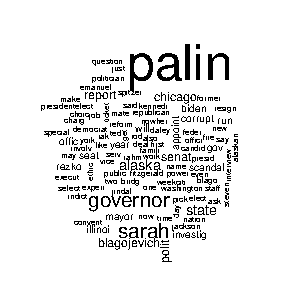
\includegraphics{stmVignette-024}
\caption{Word cloud display of vice President topic.}
\label{fig:cloud}
\end{center}
\vspace{-20pt}
\end{figure}


In addition, the Structural Topic Model permits correlations between topics. Positive correlations between topics indicate that both topics are likely to be discussed within a document. These can be visualized using \code{plot.topicCorr()}. The user can specify a correlation threshold.  If two topics are correlated above that threshold, then those two topics are considered to be linked.  After calculating which topics are correlated with one another, \code{plot.topicCorr} produces a layout of topic correlations using a force-directed layout algorithm, which we present in Figure~\ref{fig:correlations}. We can use the correlation graph to observe the connection between such as topics 12 (Iraq War) and 20 (Bush administration). \code{plot.topicCorr} has several options that are described in the help file.

\begin{Schunk}
\begin{Sinput}
R> mod.out.corr <- topicCorr(poliblogPrevFit)
\end{Sinput}
\end{Schunk}

\begin{figure}
\vspace{-20pt}
\begin{center}
\begin{Schunk}
\begin{Sinput}
R> plot.topicCorr(mod.out.corr)
\end{Sinput}
\end{Schunk}
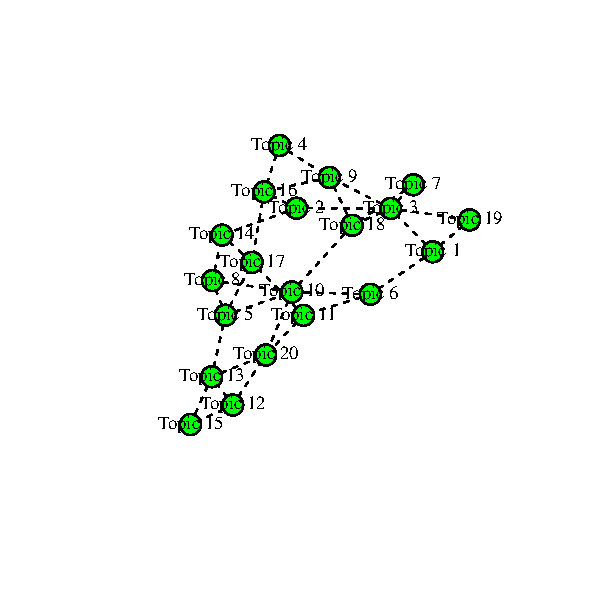
\includegraphics{stmVignette-026}
\caption{Graphical display of topic correlations.}
\label{fig:correlations}
\end{center}
\vspace{-20pt}
\end{figure}


Finally, there are several add-on packages that take output from a structural topic model and produce additional visualizations. In particular, the \pkg{stmBrowser} package contains functions to write out the results of a structural topic model to a d3 based web browser.\footnote{Available at \href{https://github.com/mroberts/stmBrowser}{https://github.com/mroberts/stmBrowser}.} The browser facilitates comparing topics, analyzing relationships between metadata and topics, and reading example documents. The \pkg{stmCorrViz} package provides a different d3 visualization environment that focuses on visualizing topic correlations using a hierarchial clustering approach that groups topics together.\footnote{Available at \href{http://cran.r-project.org/web/packages/stmCorrViz/index.html}{http://cran.r-project.org/web/packages/stmCorrViz/index.html}.} Additional packages from \texttt{R} community that leverage output from the \pkg{STM} package are welcome.
\FloatBarrier

\section{Changing basic estimation defaults}
\label{sec:defaults}

In this section, we explain how to change default settings in the \pkg{stm} package's estimation commands.  We start by discussing how to chose among different methods for initializing model parameters.  We then discuss how to set and evaluate convergence criteria.  Next we describe a method for accelerating convergence when the analysis includes a large number of documents. Finally we discuss some variations on content covariate models which allow the user to control model complexity.

\subsection{Initialization}
\label{sec:init}
As with most topic models, the objective function maximized by STM is multimodal.  This means that the way we choose the starting values for the variational EM algorithm can affect our final solution.  We provide three methods of initialization that are accessed using the argument \code{init.type}: Latent Dirichlet Allocation via collapsed Gibbs sampling (\code{init.type = "LDA"}); a Spectral algorithm for Latent Dirichlet Allocation (\code{init.type = "Spectral"}); and random starting values (\code{init.type = "Random"}).

LDA is the default option and uses several passes of collapsed Gibbs sampling to initialize the algorithm. The exact parameters for this initialization can be set using the argument \code{control}. The spectral option initializes using a moment-based estimator for LDA due to \citet{arora2012practical}. In contrast to the LDA and random initializations this approach is deterministic.  It performs extremely well particularly for larger document sets.  Because the spectral algorithm needs to form a square matrix with dimensions of the length of the vocabulary, it is best used in settings where the vocabulary is under 10,000 terms.  Finally, the random algorithm draws the initial state from a Dirichlet distribution.  The random intiailization strategy is included primarily for completeness; in general, the other two strategies should be preferred.  \citet{chaptermulti} provides details on these initialization methods and provides a study of their performance.  In general, spectral initialization outperforms LDA which in turn outperforms random initialization.

Each time the model is run, the random seed is saved in the output object under \code{settings$seed}.  This can be passed to the \code{seed} argument of \code{stm} to replicate the same starting values.


\subsection{Convergence criteria}
Estimation in the STM proceeds by variational EM.  Convergence is controlled by relative change in the variational objective.  Denoting by $\ell_t$ the approximate variational object at time $t$, convergence is declared when the quantity $(\ell_t - \ell_{t-1})/$abs($\ell_{t-1}$) drops below tolerance.  The default tolerance is 1e-5 and can be changed using the \code{emtol} argument.

The argument \code{max.em.its} sets the maximum number of iterations.  If this threshold is reached before convergence is reached a message will be printed to the screen.  The default of 500 iterations is simply a general guideline.  A model that fails to converge can be restarted using the \code{model} argument in \code{stm}.  See the documentation for \code{stm} for more information.

The default is to have the status of iterations print to the screen. The \code{verbose} option turns printing to the screen on and off.

During the E-step, the algorithm prints one dot for every $1\%$ of the corpus it completes and announces completion along with timing information.  Printing for the M-Step depends on the algorithm being used.  For models without content covariates, M-step estimation should be nearly instantaneous.  For models with content covariates, and the algorithm is set to print dots to indicate progress.  The exact interpretation of the dots differs with the choice of model (see the help file for more details).

By default every 5th iteration will print a report of top topic and covariate words.  The \code{reportevery} option sets how often these reports are printed.

Once a model has been fit, convergence can easily be assessed by plotting the variational bound as in Figure \ref{fig:converge}.

\begin{figure}
\begin{center}
\begin{Schunk}
\begin{Sinput}
R> plot(poliblogPrevFit$convergence$bound, type = "l",
+  ylab = "Approximate Objective",
+  main = "Convergence")
\end{Sinput}
\end{Schunk}
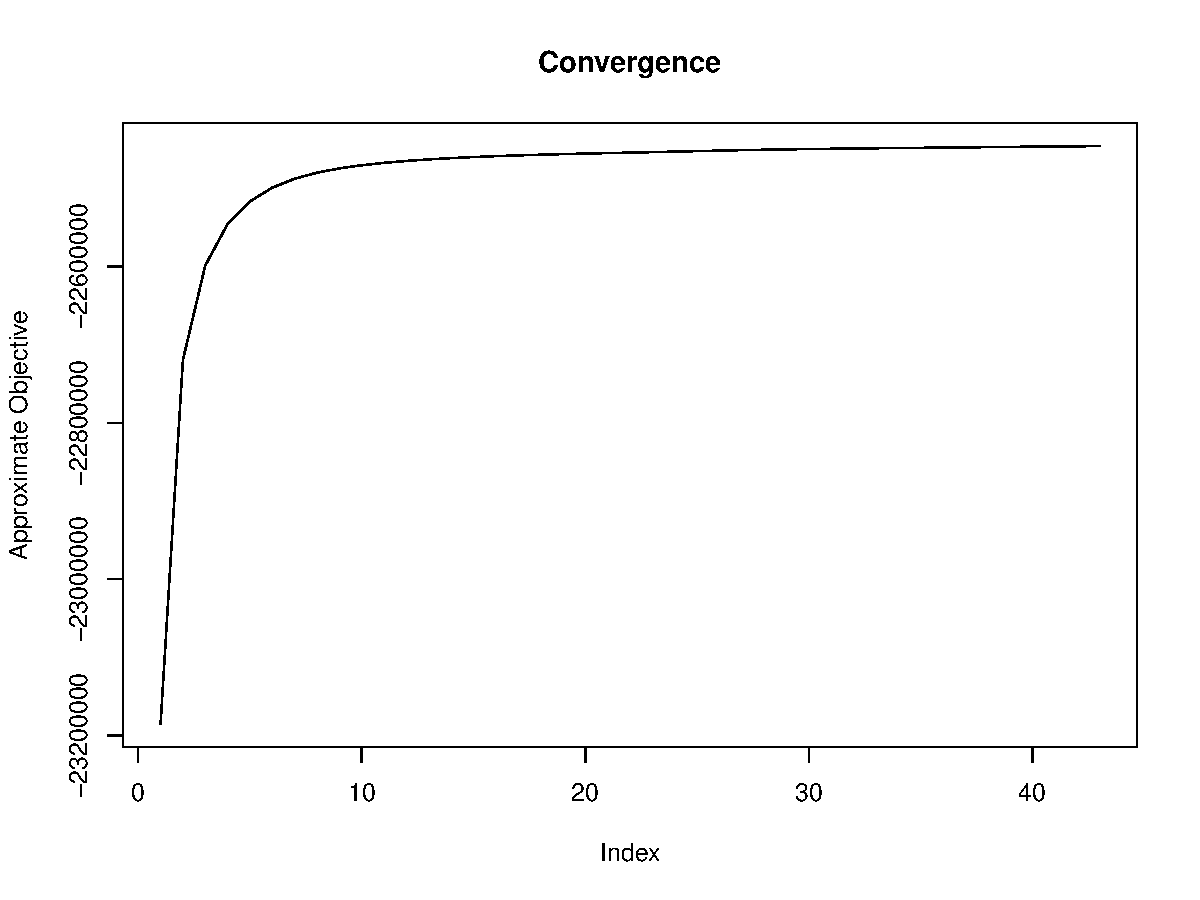
\includegraphics{stmVignette-027}
\caption{Graphical display of convergence.}
\label{fig:converge}
\end{center}
\end{figure}

\subsection{Accelerating convergence}
When the number of documents is large convergence in topic models can be slow.  This is because each iteration requires a complete pass over all the documents before updating the global parameters.  To accelerate convergence we can split the documents into several equal-sized blocks and update the global parameters after each block.  The option \code{ngroups} specifies the number of blocks, and setting it equal to an integer greater than one turns on this functionality.

Note that setting the \code{ngroups} value to a large number can dramatically increase the memory requirements of the function.  Thus as the number of blocks is increased we are trading off memory for computational efficiency.

\subsection{SAGE}
The Sparse Additive Generative (SAGE) model conceptualizes topics as sparse deviations from a corpus-wide baseline \citep{eisenstein2011sparse}.  While computationally more expensive, this can sometimes produce higher quality topics .  Whereas LDA tends to assign many rare words (words that appear only a few times in the corpus) to a topic, the regularization of the SAGE model ensures that words load onto topics only when they have sufficient counts to overwhelm the prior. In general, this means that SAGE topics have fewer unique words that distinguish one topic from another, but those words are more likely to be meaningful.  Importantly for our purposes, the SAGE framework makes it straightforward to add covariate effects into the content portion of the model.

\paragraph{Covariate-Free SAGE}
While SAGE topics are enabled automatically when using a covariate in the content model, they can also be used even without covariates.  To activate SAGE topics simply set the option \code{LDAbeta = FALSE}.

\paragraph{Covariate-Topic Interactions}
By default when a content covariate is included in the model, we also include covariate-topic interactions.  In our political blog corpus for example this means that the probability of observing a word from a Conservative blog in Topic 1 is formed by combining the baseline probability, the Topic 1 component, the Conservative component and the Topic 1 - Conservative interaction component.

Users can turn off interactions by specifying the option \code{interactions = FALSE}.  This can be helpful in settings where there isn't sufficient data to make reasonably inferences about all the interaction parameters.  It also reduces the computational intensity of the model.

\section{Alternate priors}
\label{sec:priors}

In this section we review options for altering the prior structure in the \code{stm}  function.  We highlight the alternatives and provide intuition for the properties of each option. We chose default settings that we expect will perform  the best in the majority of cases and thus changing these settings should only be necessary if the defaults are not performing well.

\subsection{Changing estimation of prevalence covariate coefficients}
The user can choose between two options: \code{"Pooled"} and \code{"L1"}.   The difference between these two is that the \code{"L1"} option can induce sparsity in the coefficients (i.e., many are set exactly to zero) while the \code{"Pooled"} estimator is computationally more efficient. \code{"Pooled"} is the default option and estimates a model where the coefficients on topic prevalence have a zero-mean Normal prior with variance given a Half-Cauchy(1,1) prior.  This provides moderate shrinkage towards zero but does not induce sparsity. In practice we recommend the default \code{"Pooled"} estimator unless the prevalence covariates are very high dimensional (such as a factor with hundreds of categories).


You can also choose \code{gamma.prior = "L1"} which uses the \code{glmnet} package \citep{friedman2010regularization} to allow for grouped penalties between the L1 and L2 norm. In these settings we estimate a regularization path and then select the optimal shrinkage parameter using a user-tunable information criterion. By default selecting the L1 option will apply the L1 penalty by selecting the optimal shrinkage parameter using AIC. The defaults have been specifically tuned for the STM but almost all the relevant arguments can be changed through the \code{control} argument. Changing the \code{gamma.enet} parameter by specifying \code{control = list(gamma.enet = .5)} allows the user to choose a mix between the L1 and L2 norms. When set to 1 (as by default) this is the lasso penalty, when set to 0 it is the ridge penalty. Any value in between is a mixture called the elastic net.

\subsection{Changing the covariance matrix prior}
The \code{sigma.prior} argument is a value between 0 and 1; by default, it is set to 0.  The update for the covariance matrix is formed by taking the convex combination of the diagonalized covariance and the MLE with weight given by the prior.  Thus by default we are simply maximizing the likelihood.  When \code{sigma.prior = 1} this amounts to setting a diagonal covariance matrix.  This argument can be useful in settings where topics are at risk of becoming too highly correlated.  However, in extensive testing we have come across very few cases where this was needed.

\subsection{Changing the content covariate prior}
The \code{kappa.prior} option provides two sparsity promoting priors for the content covariates.  The default is \code{kappa.prior = "L1"} and uses \code{glmnet} and the distributed multinomial formulation of \citet{taddy2013distributed}.  The core idea is to decouple the update into a sequence of independent L1-regularized poisson models with plugin estimators for the document level shared effects.  See \citet{stmjasa} for more details on the estimation procedure. The regularization parameter is set automatically as detailed in the \code{stm} help file.

To maintain backwards compatability we also provide estimation using a scale mixture of Normals where the precisions $\tau$ are given improper Jeffreys priors $1/\tau$. This option can be accessed by setting \code{kappa.prior = "Jeffreys"}.  We caution that this can be much slower than the default option.

There are over a dozen additional options documented in \code{stm} for altering additional components of the prior, most which focus on the content covariate model.

\section{Performance and design}
\label{sec:performance}
The primary reason to use the \pkg{stm} is the rich feature set summarized in Figure \ref{fig:stmreview}.  However, a key part of making the tool practical for every day use is increasing the speed of estimation.  Due to the non-conjugate model structure, bayesian inference for the Structural Topic Model is challenging and computationally intensive. Over the course of developing the \pkg{stm} package we have continually introduced new methods to make estimating the model faster. In this section, we demonstrate large performance gains over the closest analog accesible through \proglang{R} and then detail some of the approaches that make those gains possible.

\subsection{Benchmarks}
Without the inclusion of covariates, STM reduces to a logistic-normal topic model, often called the Correlated Topic Model (CTM) \citep{blei2007correlated}. The \pkg{topicmodels} package in \proglang{R} provides an interface to David Blei's original \proglang{C} code to estimate the CTM \citep{hornik2011topicmodels}.  This provides us with the opportunity to produce a direct comparison to a comparable model.  While the generative models are the same, the variational approximations to the posterior are actually distinct, with the Blei code using a different approach to the nonconjugacy problem.

In order to provide a direct comparison we use a set of 5000 randomly sampled documents from the poliblog2008 corpus described above.  This set of documents is included as \code{poliblog5k} in the \pkg{stm} package.  We want to evaluate both the speed with which the model estimates as well as the quality of the solution.  Due to the differences in the variational approximation the objective functions are not directly comparable so we use an estimate of the expected per-document held-out log-likelihood.  With the built-in function \code{make.heldout} we construct a dataset in which 10\% of documents have half of their words removed.  We can then evaluate the quality of inferred topics on the same evaluation set across all models.
\begin{Schunk}
\begin{Sinput}
R> set.seed(02138)
R> heldout <- make.heldout(poliblog5k.docs, poliblog5k.voc)
\end{Sinput}
\end{Schunk}
We arbitrarily decided to evaluate performance using \code{K = 100} topics.

The function \code{CTM} in the \pkg{topicmodels} package uses different default settings than the original Blei code.  Thus we present results using both sets of settings. We start by converting our document format to the simple triplet matrix format used by the \pkg{topicmodels} package using an internal \pkg{stm} function.
\begin{Schunk}
\begin{Sinput}
R> slam <- convertCorpus(heldout$documents, heldout$vocab, type="slam")
\end{Sinput}
\end{Schunk}

We then estimate the model with both sets of defaults
\begin{Schunk}
\begin{Sinput}
R> mod1 <- CTM(slam, k = 100)
R> control_CTM_VEM <- list(estimate.beta = TRUE, verbose = 1,
+  seed = as.integer(2138), nstart = 1L, best = TRUE,
+  var = list(iter.max = 20, tol = 1e-6),
+  em = list(iter.max = 1000, tol = 1e-3),
+  initialize = "random",
+  cg = list(iter.max = -1, tol = 1e-6))
R> mod2 <- CTM(slam, k = 100, control = control_CTM_VEM)
\end{Sinput}
\end{Schunk}

For the STM we estimate two versions, one with default convergence settings and one with \code{emtol = 1e-3} to match the Blei convergence tolerance.  In both cases we use the spectral initialization method which we generally recommend.
\begin{Schunk}
\begin{Sinput}
R> stm.mod1 <- stm(heldout$documents, heldout$vocab, K = 100,
+  init.type = "Spectral")
R> stm.mod2 <- stm(heldout$documents, heldout$vocab, K = 100,
+  init.type = "Spectral", emtol = 1e-3)
\end{Sinput}
\end{Schunk}

\begin{table}[]
\centering
\begin{tabular}{r|cccc}
                       & CTM & CTM (alt) & STM & STM (alt) \\
                       \hline
\# of Iterations       & 38 & 18   & 30  & 7  \\
Total Time             & 4527.1 min  & 142.6 min  & 14.3 min & 5.3 min  \\
Time Per Iteration*     & 119.1 min  & 7.9 min  & 0.5 min & 0.8 min\\
Heldout Log-Likelihood & -7.11 & -7.10 & -6.81  & -6.86
\end{tabular}
\caption{Performance Benchmarks.  Models marked with ``(alt)'' are alternate specifications with different convergence thresholds as defined in text. *Time per iteration was calculated by dividing the total run time by the number of iterations.  For CTM this is a good estimate of the average time per iteration, whereas for STM this distributes the cost of initialization across the iterations.}
\label{tab:perform}
\end{table}
We report the results in Table \ref{tab:perform}.  The results clearly demonstrate the superior performance of the \pkg{stm} implementation of the correlated topic model.  Better solutions (as measured by higher heldout log-likelihood) are found with fewer iterations and a faster runtime per iteration.  In fact, comparing comparable convergence thresholds the \pkg{stm} is able to run completely to convergence before the CTM has made a single pass through the data.

These results are particularly surprising given that the variational approximation used by STM is more involved than the one used in \cite{blei2007correlated} and implemented in \code{topicmodels}.  Rather than use a set of univariate Normals to represent the variational distribution, STM uses a Laplace approximation to the variational objective as in \cite{wang2013variational} which requires a full covariance matrix for each document.  Nevertheless, through a series of design decisions which we highlight next we have been able to speed up the code considerably.

\subsection{Design}
In \cite{blei2007correlated} and \pkg{topicmodels}, the inference procedure for each document involves iterating over four blocks of variational parameters which control the mean of the topic proportions, the variance of the topic proportions, the individual token assignments and an ancillary parameter which handles the nonconjugacy.  Two of these parameter blocks have no closed form updates and require numerical optimization.  This in turn makes the sequence of updates very slow.

By contrast in STM we combine the Laplace approximate variational inference scheme of \cite{wang2013variational} with a partially collapsed strategy inspired by \cite{khan2009variational} in which we analytically integrate out the token-level parameters. This allows us to perform one numerical optimization which optimizes the variational mean of the topic proportions ($\lambda$) and then solves in closed form for the variance and the implied token assignments.  This removes iteration between blocks of parameters within each document dramatically speeding convergence.  Details can be found in \cite{stmjasa}.

We use quasi-Newton methods to optimize $\lambda$, initializing at the previous iteration's estimate.  This process of warm-starting the optimization process means that the cost of inference per iteration often drops considerably as the model approaches convergence (e.g., the default STM example above the first iteration takes close to 45 seconds but quickly drops down to 30 seconds).    Because this optimization step is the main bottleneck for performance we code the objective function and gradient in the fast \proglang{C++} library \code{Armadillo} using the \pkg{RcppArmadillo} package \citep{RcppArmadillo}.  After computing the optimal $\lambda$ we calculate the variance of the variational posterior by calculating the hessian (also implemented in \proglang{C++}) and efficiently inverting it via the Cholesky decomposition.

The \pkg{stm} implementations also benefit from better model initialization strategies.  \pkg{topicmodels} only allows for a model to be initialized randomly or by a pre-existing model.  By contrast \pkg{stm} provides two powerful and fast initialization strategies as described above in Section \ref{sec:init}.

Numerous optimizations have been made to address models with covariates as well.  Of particular note is the use of the distributed multinomial regression framework \citep{taddy2013distributed} in settings with content covariates and an $L_1$ penalty.  This approach can often be orders of magnitude faster than the alternative.

\section{Conclusion}
\label{sec:conclusion}

The  \pkg{stm} package provides a powerful and flexible environment to perform text analysis that integrates both document metadata and topic modeling. In doing so it allows researchers understand which variables are linked with different features of text within the topic modeling framework. This paper provides an overview of how to use the features of the \pkg{stm} package, starting with ingestion, preparation, and estimation, and leading up to evaluation, understanding, and visualization. We encourage users to consult the extensive help files for more details, as well as read the companion papers that illustrate the application of this method. We also invite users to write their own add-on packages, like \pkg{stmBrowser} and \pkg{stmCorrViz}.

Furthermore, there are always gains in efficiency to be had, both in theoretical optimality and in applied programming practice.  The STM is undergoing constant streamlining and revision towards faster, more optimal computation. This includes an ongoing project on parallel computation of the STM. As corpus sizes increase, the STM will also increase in the capacity to handle more documents and more varied metadata.


\section{Appendix: Additional evaluation tools}
\label{sec:eval}

In this appendix we discuss several more advanced features of the \pkg{stm} package. Topic estimation is fundamentally imprecise, as estimation in topic model space requires both an a priori number of topics input by the user, and furthermore an optimization in a space with multiple solutions. Due to the intractability underlying the computation of topic models, we rely on external analytics of our model to understand its unique tradeoffs between competing parameters.  The \pkg{stm} package contains a variety of tools that can be used to evaluate the quality of the model as well as the user's choice of number of topics and of metadata selected for inclusion.


\subsection{Held-out likelihood estimation}
Sometimes users will want to compare model specifications to see how well each model does in predicting words within the document.  The \texttt{stm} package contains two different functions to aid with held-out likelihood estimation.  Held-out likelihood estimation is the estimation of the probability of words appearing within a document when those words have been removed from the document in the estimation step \citep{blei2003latent}.  Similar to cross-validation, when some of the data is removed from estimation and then later used for validation, the held-out likelihood helps the user assess the model's prediction performance.

We provide two different functions for the user to complete heldout likelihood estimation.  The first,  \code{make.heldout}, produces a document set where some of the words within the documents have been removed.  The user can then run a STM model on the documents with missing words.  The second, \code{eval.heldout}, evaluates the heldout likelihood for missing words based on the model run on the heldout documents.

\subsection{Residuals checks}
Users can also test the assumptions of the model within the package through the function \code{residuals}.  This function implements residual checks described in Section 4.2 of \citet{taddyestimation}, testing for overdispersion of the variance of the multinomial within the data generating process of STM.  As described in \citet{taddyestimation}, if the residuals are overdispersed, it could be that more topics are needed to soak up some of the extra variance.  While no fool-proof method has been developed to choose the number of topics, both the residual checks and held-out likelihood estimation are useful indicators of the number of topics that should be chosen.\footnote{In addition to these functions one can also explore if there words that are extremely highly associated with a single topic via the \code{checkBeta} function.}

\subsection{Checks for multi-modality}
Another diagnostic that should be completed while running the STM when not using the spectral based initializations is checking to see how multi-modal the model of interest is.  We provide a suite of methods to assess multi-modality, and we refer the reader to \citet{chaptermulti} for an explanation of all of them.  The function \code{multiSTM} aligns topics across models.  The function \code{plot.MultimodDiagnostic} plots the effects across topics and models. Both enable the researcher to investigate how different solutions lead to different inferences about the data.
 

\subsection{Post-estimation permutation checks}
Any statistical procedure can be abused and STM is no different. One concern is that users will simply search out covariate topic relationships that are the strongest. A related concern is that by combining the measurement model with the estimation of an effect, the user is ``baking in'' the conclusion. In the appendix of \cite{ajps} we address this concern using both a simulation and a permutation test approach.  We have built in a function for conducting permuation tests using binary prevalence covariates.\footnote{Future work could extend this to other types of covariates.} The \code{permutationTest} function takes a formula containing a single binary covariate (and optionally other controls) and runs a permutation test where, rather than using the true assignment, the covariate is randomly assigned to a document with probability equal to its empirical probability in the data.

After each shuffle of the covariate the same STM model is estimated at different starting values using the same initialization procedure as the original model, and the effect of the covariate across topics is calculated.
Next the function records two quantities of interest across this set of ``runs" of the model. The first quantity reports the absolute maximum effect of the permuted covariate across all topics.
The second quantity reports the effect of the (permuted) covariate on the topic in each additional STM run which is estimated to be the topic closest to the topic of interest. The object returned from \code{permutationTest} can then be passed to \code{plot.STMpermute} for plotting.




\clearpage
\pdfbookmark[1]{References}{References}
\bibliography{extracted}


\end{document}




\begin{comment}
Use of the STM typically proceeds in three key steps:

\begin{enumerate}
\item Ingest (Reading in text data) \\
(\code{textfile, corpus}, from \pkg{quanteda})
\item Process (Pre-process text data) \\
(\code{dfm}, from \pkg{quanteda})
\item Estimate (Fitting the Structural Topic Model)
(\code{stm, selectModel, manyTopics})
\item Plotting and inspecting results
(\code{plotModels},\code{plot.STM},\code{labelTopics}, \code{estimateEffect}, \code{plot.estimateEffect},\code{findThoughts}, \code{plotQuote})
\end{enumerate}
\end{comment}
